\documentclass{article} % For LaTeX2e
\usepackage{iclr2026_conference,times}

\input{math_commands.tex}

\usepackage{hyperref}
\usepackage{url}
\usepackage{graphicx}
\usepackage{booktabs}
\usepackage{amsmath,amssymb}
\usepackage{microtype}
\usepackage{subcaption}
\usepackage{enumitem}
\usepackage{array}

\title{Supplementary Material for\\A Case Study of Staged Metric-Gated GRPO for Visual Numeric Reasoning}

% Keep the real author block in source; the ICLR style will hide it in review mode
% until \iclrfinalcopy is restored.
\author{Kunal Ghosh\\
Purdue University\\
West Lafayette, Indiana, USA\\
\texttt{ghosh178@purdue.edu}\\
\texttt{kg.aero@gmail.com}}

\newcolumntype{L}[1]{>{\raggedright\arraybackslash}p{#1}}

\begin{document}

\maketitle

\section{Purpose of the Supplement}

This supplement expands the main case-study report in four directions:
\begin{enumerate}[leftmargin=1.2em]
\item the exact reward and evaluation formulas used by the repository,
\item the controller rules and checkpoint-selection logic,
\item the low-memory runtime profile used by the archived successful runs, and
\item the continuation semantics used for same-phase resume versus cross-phase warm start.
\end{enumerate}
All statements below are grounded in the following repository modules:
\begin{itemize}[leftmargin=1.2em]
\item \texttt{staged\_rl/config.py}
\item \texttt{staged\_rl/rewarding.py}
\item \texttt{staged\_rl/evaluation.py}
\item \texttt{staged\_rl/controller.py}
\item \texttt{staged\_rl/checkpointing.py}
\item \texttt{staged\_rl/trainer\_runtime.py}
\end{itemize}

\section{Background: GRPO Versus the Contribution of This Paper}

\begin{figure}[t]
\centering
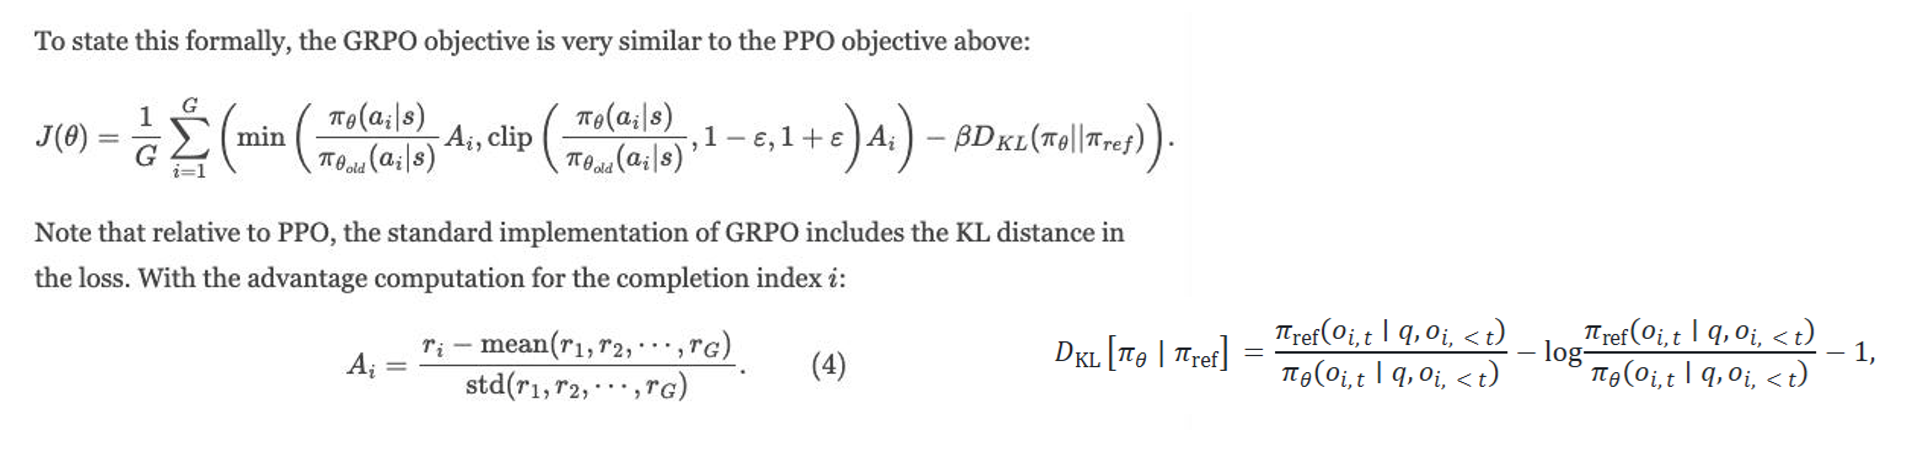
\includegraphics[width=\linewidth]{../../results/plots/GRPO.png}
\caption{Background schematic for GRPO. This figure is included only for context. The contribution of the repository analyzed in the main paper is not a new GRPO loss, but a staged controller around an existing GRPO trainer.}
\label{fig:supp-grpo}
\end{figure}

The repository uses TRL's \texttt{GRPOTrainer} as its optimization backend. The substantive contribution studied in the main report lies outside the core GRPO update:
\begin{itemize}[leftmargin=1.2em]
\item staged curriculum construction over filtered MathVista subsets,
\item a structured response contract,
\item metric-gated reward reweighting after checkpoint evaluation, and
\item alias-based checkpoint selection for continuation.
\end{itemize}
We make this distinction explicit because readers can easily conflate the optimization objective with the surrounding training stack. In this repository, the surrounding stack is the main subject of the case study.

\section{Full Reward Specification}

\begin{figure}[t]
\centering
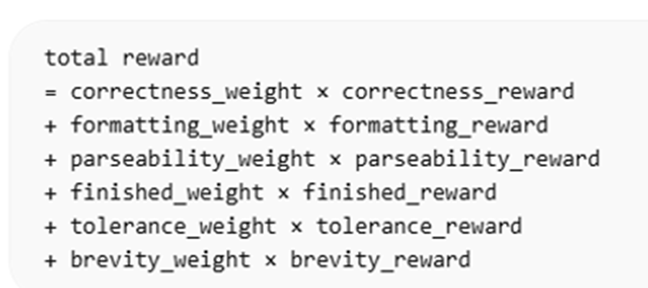
\includegraphics[width=0.68\linewidth]{../../results/plots/Reward_formula.png}
\caption{Compact visual summary of the reward decomposition used in the repository. The equations below give the exact code-aligned definition.}
\label{fig:supp-reward}
\end{figure}

Let $c$ denote a completion, $g$ the gold answer, $m \in \{\mathrm{num}, \mathrm{mc}\}$ the answer mode, and $L$ the phase-specific completion budget. Here $\mathrm{num}$ denotes the numeric free-form path and $\mathrm{mc}$ the multi-choice path. The total per-sample reward is
\begin{equation}
R(c,g,m)=
w_f R_{\mathrm{format}} +
w_p R_{\mathrm{parseable}} +
w_h R_{\mathrm{finished}} +
w_c R_{\mathrm{correctness}} +
w_b R_{\mathrm{brevity}} +
w_t R_{\mathrm{tolerance}}.
\end{equation}

\paragraph{Tag and parsing predicates.}
The implementation uses:
\begin{align}
\mathrm{ReasoningTag}(c) &= \mathbf{1}[\text{exactly one reasoning block exists}], \\
\mathrm{SolutionTag}(c) &= \mathbf{1}[\text{exactly one solution block exists}], \\
\mathrm{Malformed}(c,m) &=
\begin{cases}
\mathbf{1}[\text{numeric extraction or parsing fails}], & m=\mathrm{num},\\
\mathbf{1}[\text{option extraction fails}], & m=\mathrm{mc},
\end{cases}\\
\mathrm{Finished}(c,m) &=
\begin{cases}
1, & \mathrm{ReasoningTag}(c)=1 \wedge \mathrm{SolutionTag}(c)=1 \\
   & \wedge\ \mathrm{Malformed}(c,m)=0,\\
0, & \text{otherwise}.
\end{cases}
\end{align}

\paragraph{Reward components.}
The six reward components are:
\begin{align}
R_{\mathrm{format}}(c,m) &= \mathrm{ReasoningTag}(c) + \mathrm{SolutionTag}(c) \nonumber\\
&\quad - 0.5\,\mathrm{Malformed}(c,m),\\
R_{\mathrm{parseable}}(c,m) &=
\begin{cases}
\mathbf{1}[\text{numeric parsing succeeds}], & m=\mathrm{num},\\
\mathbf{1}[\mathrm{Malformed}(c,m)=0], & m=\mathrm{mc},
\end{cases}\\
R_{\mathrm{finished}}(c,m) &=
\begin{cases}
1, & \mathrm{Finished}(c,m)=1 \wedge \mathrm{tok}(c)<L,\\
-1, & \mathrm{tok}(c)\ge L \wedge \mathrm{Finished}(c,m)=0,\\
0, & \text{otherwise},
\end{cases}\\
R_{\mathrm{correctness}}(c,g,m) &= \mathbf{1}[\text{exact match}],\\
R_{\mathrm{brevity}}(c) &=
\begin{cases}
-1, & \mathrm{tok}(c)\ge L,\\
1, & \mathrm{tok}(c)/L \le 0.55,\\
0.5, & 0.55 < \mathrm{tok}(c)/L \le 0.75,\\
0, & 0.75 < \mathrm{tok}(c)/L \le 0.90,\\
-0.5, & 0.90 < \mathrm{tok}(c)/L < 1,
\end{cases}\\
R_{\mathrm{tolerance}}(c,g,m) &=
\begin{cases}
1, & \text{tolerance is enabled, exact match is false,}\\
   & \text{and the tolerance check holds},\\
0, & \text{otherwise}.
\end{cases}
\end{align}

Tolerance reward is active only in Phases C and D. Exact match suppresses tolerance reward, so the tolerance component acts strictly as a denser near-miss signal rather than an additional bonus for already-correct answers.

\paragraph{Phase-initialized weights.}
The configured initial weights are manual curriculum defaults rather than values learned by a meta-optimizer:
\begin{center}
\small
\begin{tabular}{lcccccc}
\toprule
Phase & Format & Parseable & Finished & Correctness & Brevity & Tolerance \\
\midrule
A & 1.0 & 1.0 & 1.5 & 2.0 & 0.25 & 0.0 \\
B & 0.75 & 0.75 & 1.0 & 4.0 & 0.20 & 0.0 \\
C & 0.50 & 0.50 & 0.75 & 5.0 & 0.20 & 1.0 \\
D & 0.50 & 0.50 & 0.75 & 5.0 & 0.30 & 1.0 \\
\bottomrule
\end{tabular}
\end{center}

\section{Evaluation Metrics and Checkpoint Scores}

For each prompt $i$, the evaluator samples one or more completions $c_{i,j}$. It computes:
\begin{align}
\mathrm{EM} &= \frac{1}{N}\sum_{i=1}^N \mathbf{1}[\text{first sampled completion matches exactly}],\\
\mathrm{TolAcc} &= \frac{1}{N}\sum_{i=1}^N \mathbf{1}[\text{first sampled completion is correct under tolerance}],\\
\mathrm{ParseRate} &= \frac{1}{M}\sum_{i,j}\mathbf{1}[\text{sample } (i,j) \text{ is parseable}],\\
\mathrm{MalfRate} &= \frac{1}{M}\sum_{i,j}\mathbf{1}[\text{sample } (i,j) \text{ is malformed}],\\
\mathrm{TruncRate} &= \frac{1}{M}\sum_{i,j}\mathbf{1}[\text{sample } (i,j) \text{ is truncated}].
\end{align}
It also computes tag-compliance rates, completion-token averages, repetition rate, sampled-answer diversity, and mean logged reward components.

The checkpoint registry then defines three scores:
\begin{align}
S_{\mathrm{struct}} &= 0.35\,\mathrm{ParseRate} + 0.20\,\mathrm{SolutionTag} \nonumber\\
&\quad + 0.20\,\mathrm{ReasoningTag} - 0.15\,\mathrm{MalfRate} \nonumber\\
&\quad - 0.10\,\mathrm{TruncRate},\\
S_{\mathrm{corr}} &= 0.70\,\mathrm{EM} + 0.20\,\mathrm{TolAcc} + 0.10\,\mathrm{ParseRate},\\
S_{\mathrm{comp}} &= 0.45\,\mathrm{EM} + 0.15\,\mathrm{TolAcc} + 0.15\,\mathrm{ParseRate} \nonumber\\
&\quad + 0.10\,\mathrm{SolutionTag} + 0.05\,\mathrm{ReasoningTag} \nonumber\\
&\quad - 0.05\,\mathrm{MalfRate} - 0.05\,\mathrm{TruncRate}.
\end{align}
These scores back the aliases \texttt{best\_structure}, \texttt{best\_correctness}, and \texttt{best\_composite}. The \texttt{latest} alias is purely chronological.

\section{Controller Rules and Thresholds}

\begin{table}[t]
\centering
\small
\caption{Controller rules implemented in \texttt{staged\_rl/controller.py}.}
\label{tab:controller-rules}
\begin{tabular}{L{0.19\linewidth} L{0.26\linewidth} L{0.41\linewidth}}
\toprule
Rule & Trigger & Action \\
\midrule
Parseable guard & parseable answer rate $< 0.85$ & Raise parseable reward to at least $0.75$ \\
Format guard & solution tag $< 0.90$ or\\ reasoning tag $< 0.88$ or\\ malformed rate $> 0.10$ & Raise format reward to at least $0.75$ \\
Finish guard & truncation rate $> 0.15$ or\\ average completion tokens exceed $0.85L$ & Add $0.25$ to finished reward \\
Stable structure test & parseable $\ge 0.92$,\\ solution $\ge 0.95$,\\ reasoning $\ge 0.93$,\\ malformed $\le 0.05$,\\ truncation $\le 0.08$ & Enable plateau-based correctness escalation once enough history exists \\
Correctness escalation & Stable structure holds over a two-checkpoint window and exact-match gain is below $0.02$ & Add $0.50$ to correctness reward \\
\bottomrule
\end{tabular}
\end{table}

The repository's controller audit covers 26 evaluated checkpoints. Across those checkpoints:
\begin{itemize}[leftmargin=1.2em]
\item parseability guard fires 2 times,
\item formatting guard fires 2 times,
\item finish guard fires 2 times,
\item correctness escalation fires 12 times, and
\item 6 correctness escalations occur when exact match has regressed rather than merely plateaued.
\end{itemize}
This behavior is consistent with the code: once the system judges structure to be stable, it reacts to weak exact-match progress by raising correctness pressure even if the immediate trend is negative.

\section{Runtime Profile and Resource-Constrained Operation}

\begin{figure}[t]
\centering
\begin{subfigure}[t]{0.49\linewidth}
\centering
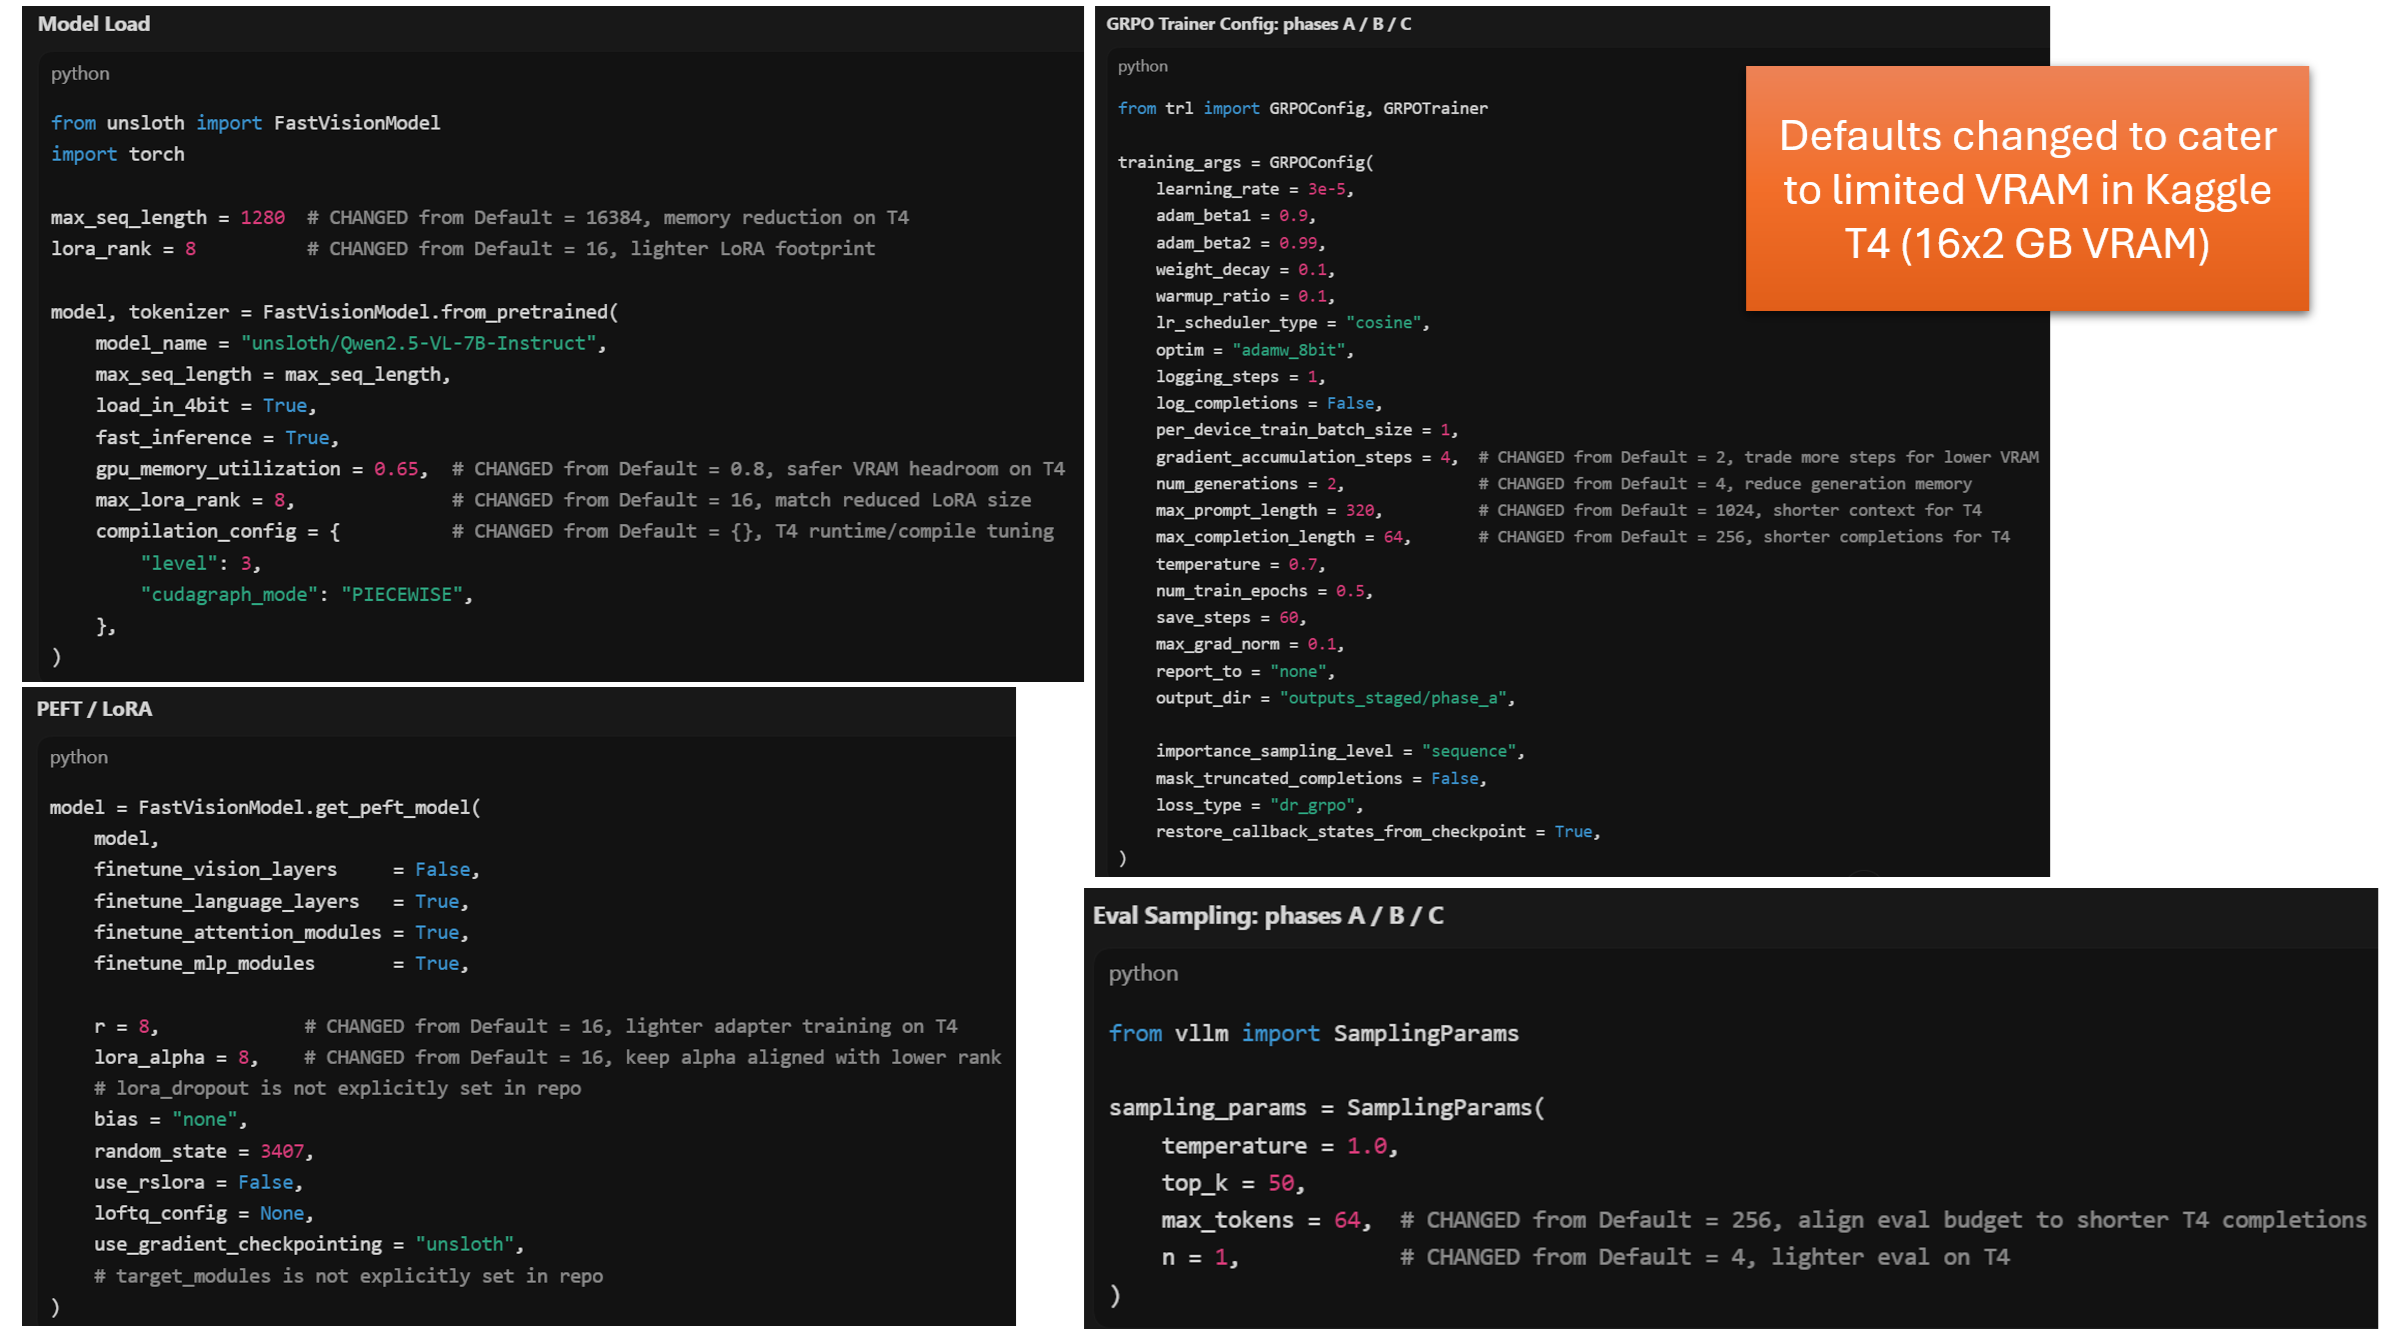
\includegraphics[width=\linewidth]{../../results/plots/Parameter_changes.png}
\caption{Primary hardware-profile changes.}
\end{subfigure}
\hfill
\begin{subfigure}[t]{0.49\linewidth}
\centering
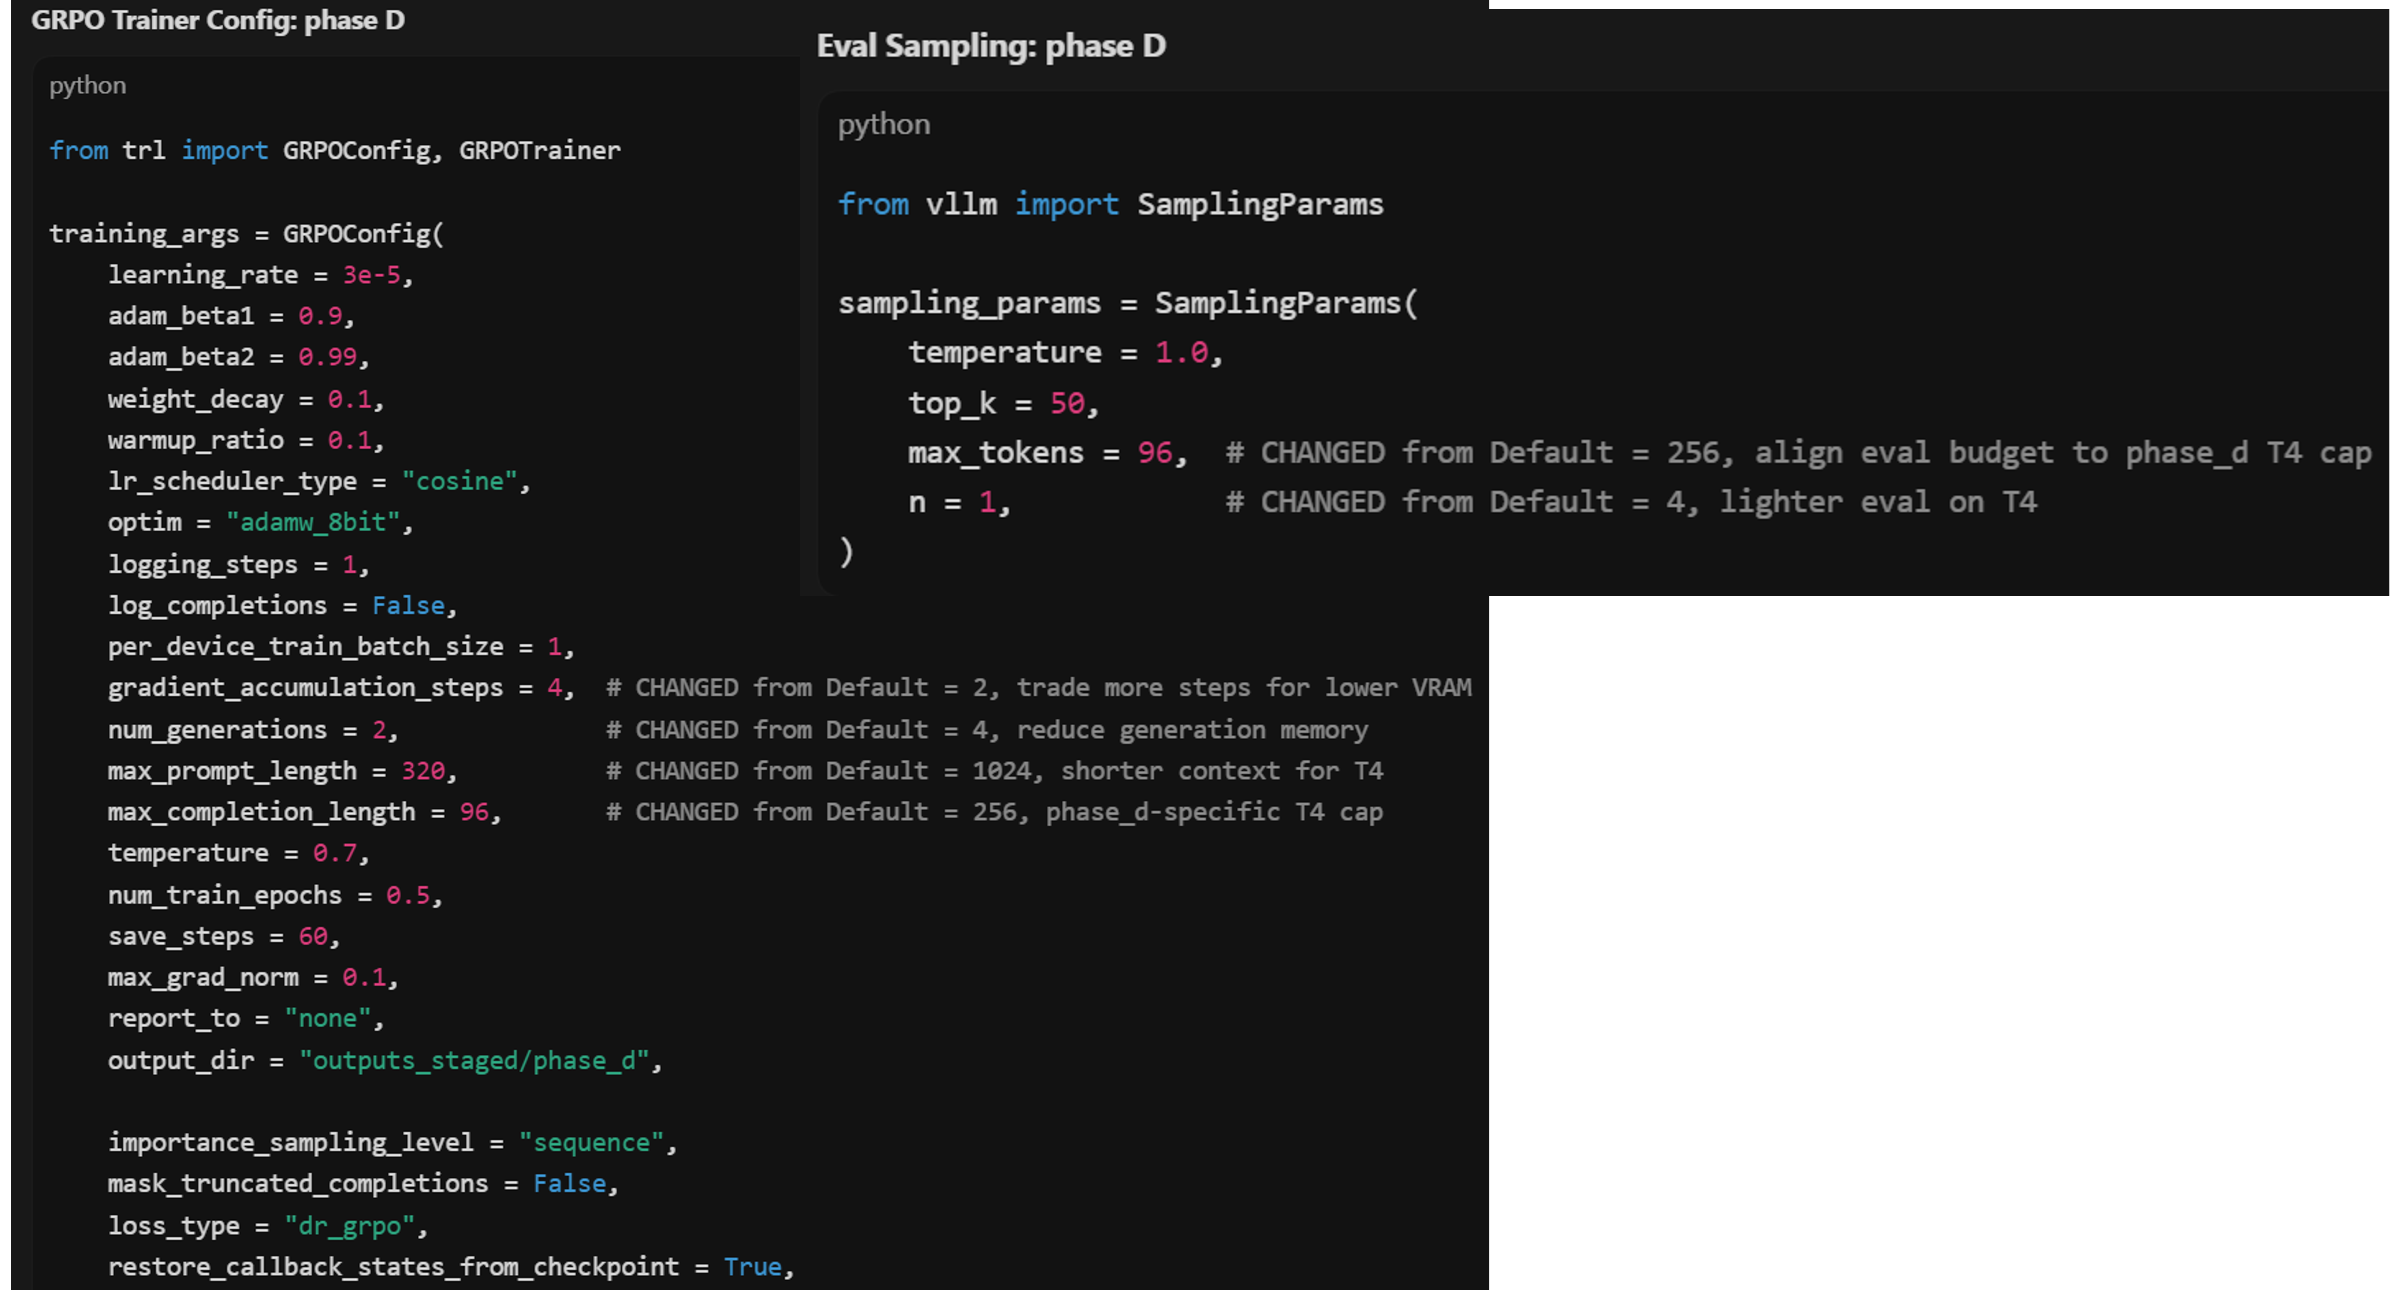
\includegraphics[width=\linewidth]{../../results/plots/Parameter_changes_2.png}
\caption{Secondary and phase-specific changes.}
\end{subfigure}
\caption{Supporting figures for the repository's conservative Kaggle T4 profile.}
\label{fig:supp-params}
\end{figure}

The archived successful runs share the same low-memory profile:
\begin{itemize}[leftmargin=1.2em]
\item max sequence length reduced from $16384$ to $1280$,
\item image size reduced from $512$ to $336$,
\item LoRA rank reduced from $16$ to $8$,
\item sampled generations reduced from $4$ to $2$,
\item max prompt length reduced from $1024$ to $320$,
\item max completion length reduced from $256$ to $64$ in the default Kaggle profile,
\item max completion length increased to $96$ only for Phase D,
\item evaluation reduced to one sample per prompt and at most two examples per subset.
\end{itemize}
The repository interprets these changes as runtime stabilizers rather than task simplifiers. They reduce per-step VRAM pressure and evaluation overhead, but they also reduce reasoning budget, visual detail, and generation diversity.

\section{Transfer and Continuation Semantics}

The code distinguishes three different mechanisms that can be conflated in informal descriptions:
\begin{enumerate}[leftmargin=1.2em]
\item \textbf{Cross-notebook transfer.} A checkpoint directory is physically moved through a Kaggle dataset attachment or another external bundle.
\item \textbf{Warm start.} A fresh base model is loaded, a fresh LoRA adapter is attached, and adapter weights are copied from the selected checkpoint into that new adapter.
\item \textbf{Same-phase resume.} Full trainer state is restored from a checkpoint, including optimizer state, scheduler state, trainer progress, and controller state.
\end{enumerate}

This distinction matters for the report's claims. Cross-phase continuation often uses alias-based warm start, not exact trainer resume. Same-phase restarts can use exact trainer resume if the selected checkpoint belongs to the current phase.

\section{Additional Notes on Scope}

The repository contains scaffolding for a multi-choice branch and an optional robustness stage, but neither path provides the main evidence used in the report. Similarly, the runner logs when multiple GPUs are visible but does not automatically switch to DDP or tensor parallelism. The strongest claims are therefore:
\begin{itemize}[leftmargin=1.2em]
\item about staged RL dynamics for numeric visual reasoning,
\item about metric-gated control under non-monotonic checkpoint trajectories, and
\item about making a single-GPU GRPO pipeline more auditable and reproducible.
\end{itemize}

\end{document}
